%%%%%%%%%%%%%%%%%%%%%%%%%%%%%%%%%%%%%%%%%%%%%%%%%%%%%%%%%%%%%%%%%%%%%%%%%%%%%%%%
%%
%% Шаблон диссертации
%%
%%%%%%%%%%%%%%%%%%%%%%%%%%%%%%%%%%%%%%%%%%%%%%%%%%%%%%%%%%%%%%%%%%%%%%%%%%%%%%%%

%%%%%%%%%%%%%%%%%%%%%%%%%%%%%%%%%%%%%%%%%%%%%%%%%%%%%%%%%%%%%%%%%%%%%%%%%%%%%%%%
%%
%% All LaTeX characters appearing in this dissertation are fictitious.
%% Any resemblance to real dissertations, published or not, is purely coincidental.
%%
%%%%%%%%%%%%%%%%%%%%%%%%%%%%%%%%%%%%%%%%%%%%%%%%%%%%%%%%%%%%%%%%%%%%%%%%%по%%%%%%%

\documentclass[%
  a5paper,
  subf,
  href,
  master,
  dotsinheaders 
]{csse-fcs}

\usepackage[T2A]{fontenc}
\usepackage[utf8]{inputenc}
\usepackage[english,russian]{babel}

\usepackage{cmap} % чтобы работал поиск по PDF

% Компактные списки
\usepackage{mdwlist}

% Таблицы
\usepackage{array}

% Листинги
\usepackage{listings}

% TODOs
\usepackage[%
  colorinlistoftodos,
  shadow
]{todonotes}

% Путь к каталогу со всеми рисунками
\graphicspath{{fig/}}

% Автоконвертер для EPS
% \usepackage{epstopdf}

% Генератор текста
\usepackage{blindtext}

\usepackage{nomencl}
\usepackage{tabu}
\usepackage{float}

% Для таблиц с объединенными ячейками
\usepackage{multirow}

% Полуторный интервал
\usepackage{setspace}
\onehalfspacing

\usepackage{tikz}
\usepackage{tcolorbox}
\usetikzlibrary{calc, chains, positioning, fit, arrows, shapes, automata}
\newcommand{\empt}[2]{$#1^{\langle #2 \rangle}$}

\usepackage{cite}
% \usepackage{subcaption}
\usepackage{hhline}
\usepackage{color}

\usepackage{graphicx}

\pdfimageresolution=300

%%%%%%%%%%%%%%%%%%%%%%%%%%%%%%%%%%%%%%%%%%%%%%%%%%%%%%%%%%%%%%%%%%%%%%%%%%%%%%%%

\begin{document}

% \captionsetup{justification=justified}

%%%%%%%%%%%%%%%%%%%%%%%%%%%%%%%%%%%%%%%%%%%%%%%%%%%%%%%%%%%%%%%%%%%%%%%%%%%%%%%%
 
% Быть посвободнее при склеивании слов
\sloppy

\definecolor{lightgray}{rgb}{.9,.9,.9}
\definecolor{darkgray}{rgb}{.4,.4,.4}
\definecolor{purple}{rgb}{0.65, 0.12, 0.82}

% Настройка листингов
\renewcommand{\lstlistingname}{Листинг}
% \lstset{
% 	frame=single, % adds a frame around the code
% 	rulesepcolor=\color{gray},
% 	rulecolor=\color{black},
% 	breaklines=true,
% 	xleftmargin=2em,
% 	extendedchars={true},
% 	inputencoding={utf8},
% 	basicstyle={\ttfamily \scriptsize},
% 	keywordstyle={\rmfamily \bfseries},
% 	commentstyle={\rmfamily \itshape},
% 	tabsize={2},
% 	numbers={left},
% 	frame={single},
% 	showstringspaces={false},
% }

\DeclareFixedFont{\ttb}{T1}{txtt}{bx}{n}{8} % for bold
\DeclareFixedFont{\ttm}{T1}{txtt}{m}{n}{8}  % for normal

% Custom colors
\definecolor{deepblue}{rgb}{0,0,0.5}
\definecolor{deepred}{rgb}{0.6,0,0}
\definecolor{deepgreen}{rgb}{0,0.5,0}

\lstdefinelanguage{JavaScript}{
  keywords={typeof, new, catch, function, return, null, catch, var, if, in, while, do, else, case, break, try, switch, route, paper, ContentCourse, EditCourse},
  keywordstyle=\color{blue}\bfseries,
  ndkeywords={class, module, boolean, throw, implements, import, this, const, from, run, add, workdir, env, ENTRYPOINT},
  ndkeywordstyle=\color{purple}\bfseries,
  otherkeywords={require},
  %otherkeywordstyle=\color{purple}\bfseries,
  identifierstyle=\color{black},
  sensitive=false,
  comment=[l]{//},
  morecomment=[s]{/*}{*/},
  commentstyle=\color{darkgray}\ttfamily,
  stringstyle=\color{deepgreen}\ttfamily,
  morestring=[b]',
  morestring=[b]"
}

\lstset{
   	language=JavaScript,
	basicstyle={\ttfamily\scriptsize},        
	emphstyle=\color{deepred},   
	frame=tb,                         
	showstringspaces=false,             
	breaklines=true,
}


\lstset{
    literate={а}{{\selectfont\char224}}1
    {б}{{\selectfont\char225}}1
    {в}{{\selectfont\char226}}1
    {г}{{\selectfont\char227}}1
    {д}{{\selectfont\char228}}1
    {е}{{\selectfont\char229}}1
    {ё}{{\"e}}1
    {ж}{{\selectfont\char230}}1
    {з}{{\selectfont\char231}}1
    {и}{{\selectfont\char232}}1
    {й}{{\selectfont\char233}}1
    {к}{{\selectfont\char234}}1
    {л}{{\selectfont\char235}}1
    {м}{{\selectfont\char236}}1
    {н}{{\selectfont\char237}}1
    {о}{{\selectfont\char238}}1
    {п}{{\selectfont\char239}}1
    {р}{{\selectfont\char240}}1
    {с}{{\selectfont\char241}}1
    {т}{{\selectfont\char242}}1
    {у}{{\selectfont\char243}}1
    {ф}{{\selectfont\char244}}1
    {х}{{\selectfont\char245}}1
    {ц}{{\selectfont\char246}}1
    {ч}{{\selectfont\char247}}1
    {ш}{{\selectfont\char248}}1
    {щ}{{\selectfont\char249}}1
    {ъ}{{\selectfont\char250}}1
    {ы}{{\selectfont\char251}}1
    {ь}{{\selectfont\char252}}1
    {э}{{\selectfont\char253}}1
    {ю}{{\selectfont\char254}}1
    {я}{{\selectfont\char255}}1
    {А}{{\selectfont\char192}}1
    {Б}{{\selectfont\char193}}1
    {В}{{\selectfont\char194}}1
    {Г}{{\selectfont\char195}}1
    {Д}{{\selectfont\char196}}1
    {Е}{{\selectfont\char197}}1
    {Ё}{{\"E}}1
    {Ж}{{\selectfont\char198}}1
    {З}{{\selectfont\char199}}1
    {И}{{\selectfont\char200}}1
    {Й}{{\selectfont\char201}}1
    {К}{{\selectfont\char202}}1
    {Л}{{\selectfont\char203}}1
    {М}{{\selectfont\char204}}1
    {Н}{{\selectfont\char205}}1
    {О}{{\selectfont\char206}}1
    {П}{{\selectfont\char207}}1
    {Р}{{\selectfont\char208}}1
    {С}{{\selectfont\char209}}1
    {Т}{{\selectfont\char210}}1
    {У}{{\selectfont\char211}}1
    {Ф}{{\selectfont\char212}}1
    {Х}{{\selectfont\char213}}1
    {Ц}{{\selectfont\char214}}1
    {Ч}{{\selectfont\char215}}1
    {Ш}{{\selectfont\char216}}1
    {Щ}{{\selectfont\char217}}1
    {Ъ}{{\selectfont\char218}}1
    {Ы}{{\selectfont\char219}}1
    {Ь}{{\selectfont\char220}}1
    {Э}{{\selectfont\char221}}1
    {Ю}{{\selectfont\char222}}1
    {Я}{{\selectfont\char223}}1
}
 

%%%%%%%%%%%%%%%%%%%%%%%%%%%%%%%%%%%%%%%%%%%%%%%%%%%%%%%%%%%%%%%%%%%%%%%%%%%%%%%%

%\listoftodos
%\clearpage

%%%%%%%%%%%%%%%%%%%%%%%%%%%%%%%%%%%%%%%%%%%%%%%%%%%%%%%%%%%%%%%%%%%%%%%%%%%%%%%%

% Заведующий кафедрой
\apname{В.М.~Ицыксон}

% Название
\title{%
%ВЫПУСКНАЯ КВАЛИФИКАЦИОННАЯ РАБОТА БАКАЛАВРА
\textsc{выпускная квалификационная работа бакалавра}
}

% Тема
\topic{%
Разработка веб-приложения для управления контентом мобильной среды для изучения интонации.}

% Направление
\coursenum{09.03.01}
\course{Информатика и вычислительная техника}
\masterprognum{09.03.01\_02}
\masterprog{Технологии разработки программного 
обеспечения}
 
% Автор
\author{М.С.~Мальцев}
\group{43501/3~}

% Научный руководитель
\sa{Н.В.~Богач}
\sastatus{к.~т.~н.,~доц.}

% Рецензент
% \rev{Р.Е.~Цензент}
% \revstatus{к.~т.~н.,~доц.}

% Консультант
% \conspec{нормоконтролю}
% \con{А.Г.~Новопашенный}
% \constatus{к.~т.~н.,~доц.}

% Уменьшить размер шрифта для названия института, так как он не влезает в
% одну строчку по новому размеру страницы
\renewcommand\instfont{\small}
% Переопределение названий Университета/Факультета/Кафедры
%\institution{Усть-Гатчинский государственный университет кирпично-велосипедной 
%промышленности}
%\faculty{Институт кройки и шитья}
%\department{Кафедра построения конструкций из пластилина}

% \logo{fig/spbpu.jpg}


%%%%%%%%%%%%%%%%%%%%%%%%%%%%%%%%%%%%%%%%%%%%%%%%%%%%%%%%%%%%%%%%%%%%%%%%%%%%%%%%

\makecover
\maketitle 

%%%%%%%%%%%%%%%%%%%%%%%%%%%%%%%%%%%%%%%%%%%%%%%%%%%%%%%%%%%%%%%%%%%%%%%%%%%%%%%%

\blankpagecontent{ }
\makeblankpage

%%%%%%%%%%%%%%%%%%%%%%%%%%%%%%%%%%%%%%%%%%%%%%%%%%%%%%%%%%%%%%%%%%%%%%%%%%%%%%%%

\keywords{%
 Разработка веб-приложения для управления контентом мобильной среды для изучения интонации.
}

\abstractcontent{
В работе рассматривается проектирование и разработка веб-приложения для управления контентом мобильной среды для изучения интонации. Изучение интонации - важная часть изучения языка, но на сегодняшний день не существует законченных свободно распространяемых продуктов, которые позволяли бы их изучать. Разрабатываемое веб-приложение является частью проекта “Study Intonation”, который ставит целью создать открытую среду для изучения интонаций.

Мотивация разработки приложения - предоставить пользователям проекта “Study Intonation” возможность создавать, редактировать и распространять курсы в удобной форме. Также в мотивацию включена цель изучить используемый технологический стек и полный процесс создания одностраничного веб-приложения.

Работа сконцентрирована вокруг проектирования и реализации веб-прило­жения. При проектировании выделено 5 компонентов: клиентская часть, серверная часть, база данных, упаковщик и файловое хранилище. В качестве технологического стека выбран MERN + AWS S3. Разработанные компоненты размещены в Docker-контейнерах.
}

\makeabstractru

%%%%%%%%%%%%%%%%%%%%%%%%%%%%%%%%%%%%%%%%%%%%%%%%%%%%%%%%%%%%%%%%%%%%%%%%%%%%%%%%

\tableofcontents

%%%%%%%%%%%%%%%%%%%%%%%%%%%%%%%%%%%%%%%%%%%%%%%%%%%%%%%%%%%%%%%%%%%%%%%%%%%%%%%%
% 
% \makenomenclature
% \printnomenclature

%%%%%%%%%%%%%%%%%%%%%%%%%%%%%%%%%%%%%%%%%%%%%%%%%%%%%%%%%%%%%%%%%%%%%%%%%%%%%%%%

\intro

Благодаря появлению и развитию современных информационно-коммуникационных технологий сформировалась совершенно новая область в сфере образования - электронное обучение. Такая точка зрения подкрепляется работами \cite{goyal2012learning, jethro2012learning}, в которых представлены рассуждения о будущем образования и эффективном обучении.

В работах \cite{pravodelov2015, borodickaya2017, alonceva2018creating, vaganova2017elecrt}, которые освещают аспекты дистанционного обучения, в качестве ключевых преимуществ электронного обучения для слушателей выделяется: гибкость, доступность и самоорганизованность. А для преподавателей: низкая себестоимость и возможность привлечения большой аудитории.

Электронное обучение, несет в себе не только количественное улучшение существующей системы, но и качественное. Например, в работе \cite{yarasheva2014}, посвященной информационным технологиям в обучении иностранному языку, утверждается:
“Под применением новых информационных технологий в обучении иностранным языкам понимают не только использование современных технических средств и технологий, но и использование новых форм и методов преподавания иностранного языка и новый подход к процессу обучения в целом.”.

Таким образом, определяется вектор изменений, который несёт в себе многогранное улучшение образовательной системы.

В качестве проекта, который не просто переводит процесс изучения языков в интернет пространство, а предлагает новый способ освоения языка, через изучение интонации, выступает “Study Intonation” - мобильная среда для изучения интонаций \cite{lezhenin2017study}. Проект состоит из двух частей: мобильное приложение для работы с курсами и веб-приложение для их создания. В задачи мобильного приложения входит загрузка курсов и обеспечение взаимодействия с пользователем: запись речи пользователя, вычисление метрики соответствия между интонацией обучающегося и эталонным значением, которое заложено в курсе, и вывод результатов для корректировки произношения.

В данной работе акцент сделан на разработке веб-приложения для создания, редактирования и распространения курсов. Работа сконцентрирована вокруг проектирования и реализации веб-приложения.

Мотивация разработки приложения - предоставить пользователям проекта “Study Intonation” возможность создавать, редактировать и распространять курсы в удобной форме. Также в мотивацию включена цель изучить используемый технологический стек и полный процесс создания одностраничного веб-приложения.

Для создания веб-приложения используется стек MERN (MongoDB, Express, React, Node.js). MongoDB - документоориентированная СУБД. Node.js - программная платформа позволяющая запускать JavaScript вне браузера. Express - минималистичный и гибкий веб-фреймворк для приложений Node.js, предоставляющий обширный набор функций для мобильных и веб-приложений. React - JavaScript-библиотека для создания пользовательского интерфейса.
Для размещения медиафайлов используется файловое хранилище реализующее интерфейс AWS S3. Разработанные компоненты размещены в Docker-контейнерах и запускаются с помощью Docker Compose.


\chapter{Анализ}
 
В главе описано позиционирование разрабатываемого продукта, необходимость применения собственного решения, а также функциональные и нефункциональные требования, предъявляемые к разрабатываемому продукту.
 
\section{Обзор предметной области}

В современном интернет пространстве большая часть контента, создается пользователями. Именно на этом принципе построена парадигма Web 2.0. Термин Web 2.0 описывает второе поколение WWW, которое отличается от первого поколения более высокой интерактивностью и динамичностью, а также фокусируется на пользователях и их способностях объединяться в сообщества и делиться информацией \cite{techopedia}. С рассматриваемым термином связаны такие понятия, как обмен, коллаборации, социализация, однако, ключевым преимуществом Web 2.0 является возможность использовать коллективный интеллект, для формирования контента, наполняющего интернет пространство. Хотя изначально Web 2.0 не был предназначен для образовательных целей, он отлично справляется с задачами личностного и профессионального развития. Например, в работе \cite{franklin2007web} отмечается высокий потенциал в использовании технологий Web 2.0 для образовательной сферы.

Если же рассматривать более узкую область применения рассматриваемых технологий, а именно, изучение иностранных языков, то и в данном случае, Web 2.0 хорошо себя зарекомендовал. В работе \cite{bacsal2014using} говорится, что преподаватели иностранных языков особенно заинтересованы в новых технологиях, которые позволят учащимся улучшить их языковые навыки.

Таким образом, идея использования принципов Web 2.0 в проекте “Study Intonation” полностью обоснована.

Важным остается место педагога в новой среде. В работе \cite{yengin2010roles} в качестве одной из основных задач, которые остаются за преподавателем, выделяется создание онлайн курсов. Но существуют сложности связанные с тем, что не все учителя умеют пользоваться новыми технологиями, о них упоминается в статьях \cite{huang2008web, pushpanathanrole}. Преподавателям необходимо адаптироваться к новому интернет поколению, которое с детства обладает навыками работы с компьютерами, и корректировать свои методики обучения для более эффективного их применения \cite{tenegen}.

Для того, чтобы помочь преподавателям сориентироваться в современных технологиях и способах их применения были организованы такие проекты, как “SLOOP”, “Tenegen” \footnote{http://tenegen.eu/}, позже “Sloop2desc” \footnote{http://www.sloop2desc.eu/}, в России - проект “ШЛЮПА”. Идея проектов заключалась в том, чтобы “применить философию бесплатного программного обеспечения к производству педагогических материалов для электронного обучения” \cite{shlupa}. Но, к сожалению, все перечисленные выше проекты прекратили свое существование. “Study Intonation” поддерживает подобную философию и основывается на похожих принципах.

При рассмотрении современных средств для изучения иностранных языков, находящихся в свободном доступе, следует отметить что большая часть из них нацелена на расширение словарного запаса и объяснение грамматических основ языка, а сами системы в своем большинстве закрыты для добавления обучающего контента, создаваемого пользователями. Если же такая функция имеется, то обычно она является платной. Подобный подход, безусловно, является коммерчески обоснованным, но, таким образом, он нарушает идею свободного электронного обучения.

Интонации  играют важную роль в разговорной речи человека. Например, в работе \cite{luciasvalls}, посвященной проблеме преподавания интонаций, говорится о том, что в некоторых случаях интонации несут больше информации, чем слова. Однако на изучение интонаций в преподавании языков отводится не так много времени. О важности изучения интонаций пишут в статье \cite{taskdiscourse}. В ней автор рассуждает над тем, стоит ли вообще преподавать интонации, и приходит к выводу, что для более успешного освоения языка интонации необходимы.

На данный момент не существует свободно распространяемого законченного продукта, который бы предлагал изучать иностранные языки делая при этом акцент на интонациях, а следовательно и ни одного ресурса, который бы позволял создавать курсы для подобной задачи. В статье \cite{pennington2019using} приводится несколько приложений, который ставят перед собой похожие задачи, но они обладают скудной функциональностью и распространяются платно. Именно подобная проблема ставит задачу разработки собственного решения. Кроме того, стоит отметить, что мобильное приложение для изучения иностранных языков уже создано и на момент написания работы находится на этапе бета-тестирования, а, следовательно, формат задания курсов уже определен

Структура курсов состоит из JSON-файла, медиафайлов и файлов с отсчетами питча.
В JSON-файле содержится описание курса, а также уроков и задач, из которых состоит курс, также в нём присутствуют ссылки на файлы, которые используются в курсе.

Несколько уже созданных курсов формировались вручную, т.е. пользователь, создающий контент, с помощью примитивного текстового редактора формировал JSON-файл и по указанным в нём ссылкам размещал необходимые файлы. Подобный способ формирования контента является не удобным для пользователей по ряду причин: 

\begin{enumerate}
  \item ошибки, допущенные при формировании, курса сложно отслеживать и исправлять
  \item формат используемого JSON-файла понятен не всем пользователям
\end{enumerate}

Исходя из этих предпосылок было решено разработать сервис, который позволит в удобном формате создавать, редактировать и распространять контент для мобильной среды.


\section{Функциональные требования к архитектуре}

Необходимо создать систему, которая позволяет создать, редактировать и распространять курсы для изучения языков с акцентом на интонациях. Система должна представлять графический интерфейс и обеспечивать доступ к нему с помощью браузера. Пользователь использующий приложение, должен иметь доступ к уже существующим курсам. Возможность зарегистрироваться, если же он ранее был зарегистрирован, то войти в систему. После аутентификации, должна открываться возможность создать новый курс, а также редактировать курсы ранее добавленные этим пользователем.


При создании и редактировании курса должна быть реализована возможность ввода названия, описания, уровня сложности, категории, и указания авторов, а также загрузки изображения в форматах *.jpg и *.png для обложки курса.

При создании урока или его редактирования пользователю должны быть доступны поля: название, описание, номер, длительность.
При создании и редактировании заданий необходимо обеспечить возможность заполнения полей: 
номер, инструкции пользователю и текст задания. Должна быть реализована возможность загрузки аудиофайлов в форматах *.wav и *.mp3, а также вычисления по аудиофайлу питча и сохранения его в отдельном файле с расширением *.pitch.

Также по запросу пользователям система должна организовывать архивирование JSON-файла и медиафайлов, относящихся к выбранному курсу, с последующим размещением его для дальнейшего скачивания. При этом должен быть доступен для скачивания JSON-файл, который содержит краткое описание курсов для уведомления мобильного клиента о новых и обновленных курсах.

\section{Нефункциональные требования к архитектуре}

Разрабатываемое приложение должно удовлетворять следующим нефункциональным требованиям:

\begin{itemize}
	\item Приложение должно обеспечивать правильное отображение сайта на различных устройствах, подключенных к интернету, и динамически подстраивающийся под заданные размеры окна браузера
	\item Разрабатываемый графический интерфейс должен демонстрировать высокие пользовательские качества
	\item Продукт должен легко масштабироваться без серьезных изменений в коде 
	\item Приложение должно легко запускаться и разворачиваться, на не специализированом хостинге
\end{itemize}

\section{Результаты}

В результате анализа предметной области сделан вывод, что при изучении иностранных языков подход основанный на интонациях обоснован. Аналогов для проекта “Study Intonation” почти нет, а те что есть предоставляют скудную функциональность и распространяются платно. Как следствие, сервисы, позволяющие создавать курсы подобного типа, тоже отсутствуют. А также в условиях уже существующего мобильного приложения, необходима разработка своего собственного продукта, который будет позволять создавать, редактировать и распространять контент для мобильной среды. Описаны функциональные и нефункциональные требования к разрабатываемому веб-приложению.

\chapter{Проектирование}

В главе описано проектирование архитектуры приложения. Определены взаимоотношения между компонентами и технологический стек. 

% \section{Выбор инструментов}

\section{Архитектура}

Архитектура разрабатываемого приложения состоит из 5 частей:

\begin{itemize}
	\item база данных
	\item сервер
	\item клиент
	\item файловое хранилище
	\item упаковщик
\end{itemize}

\begin{figure}[H]
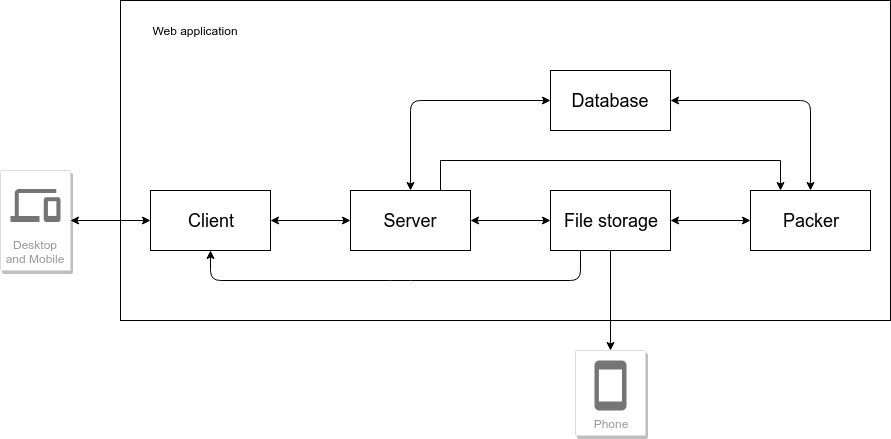
\includegraphics[width=1\textwidth]{img/1.png}
\captionsetup{justification=justified}
\caption{Архитектура разрабатываемого приложения. Компоненты и взаимоотношения между ними. }
\label{architecture_comp}
\end{figure}

К преимуществам подобного разделения относится легкая масштабируемость системы, так как при увеличении нагрузки на один из компонентов его можно заменить другим, более производительным. Например, при увеличении количества медиафайлов, размещающихся на файловом хранилище, можно сменить его, купив больший объем пространства, при этом остальные компоненты системы останутся неизменными. Причем подобные операции можно совершать над любым из компонентов. В качестве преимущества используемого подхода стоит упомянуть надежность системы. В случае отказа серверной части приложения, файловое хранилище все еще будет доступно, и пользователи смогут скачать курсы, необходимые для работы мобильного приложения. В следующих подпунктах каждый из компонентов, его назначение и функции описаны отдельно.


\subsection{База данных}

База данных хранит информацию о пользователях и курсах. Первоначально планируется небольшое количество пользователей, примерно от 100 до 1000. Однако структура курсов предполагается довольно объёмной. В один курс может входить более 15 уроков и в каждом уроке около 20 заданий. Учитывая, что у пользователей может быть по несколько созданных курсов, объем данных предполагается средний. Но если учесть, что при поддержке приложения структура курса может измениться, наиболее удачным выбором системы управления базами данных будет NoSQL решение. Подобные базы данных не имеют четкой структуры, что позволит изменять схему курса без вреда уже существующим наработкам.

\subsection{Серверная часть}

Серверная часть веб-приложения решает такие задачи, как получение запросов с клиентской части, их обработка и ответ, заключающийся в отправке клиенту запрашиваемой информации в JSON формате. Сервер имеет доступ к базе данных и файловому хранилищу. 

В данном случае не требуется какой-то сложной функциональности со стороны сервера, помимо вычисления питча. Но и эту задачу на себя берёт сторонняя библиотека на С++. Следовательно, наиболее релевантным в данном случае будет выбор технологии, которая позволит максимально просто создать веб-сервер, который будет легко взаимодействовать с NoSQL базой данных, файловым хранилищем и без особых сложностей сможет вызвать нативный код, написанный на C++.

\subsection{Клиентская часть}

В задачи решаемые клиентской частью веб-приложения входит представление пользователю графического интерфейса для визуализации информации приходящей с серверной части веб-приложения, фиксация действий пользователя и уведомление о них серверной части. Стоит отметить, что клиентская часть веб-приложения выполняется в веб-браузере пользователя. Так как предполагается, что пользователи будут создавать и редактировать курсы, уроки и задания, то ожидаемо частое обновления контента на веб-странице, как следствие, наиболее оптимальным решением будет выбрать одностраничную архитектуру приложения, так как она позволяет обновлять не всю веб-страницу целиком, а лишь изменившиеся ее части.

\subsection{Файловое хранилище}

Файловое хранилище необходимо для размещения курсов пользователей. Использование хранилища обеспечивает надежность веб-приложения, в случае если сервер откажет, так как доступ к скачиванию курсов на мобильное устройство всё ещё будет открыт. Предполагается использовать сервис реализующий Amazon S3 протокол, так как в случае критичного увеличения объема данных, которые необходимо хранить, появляется возможность перенести файловое хранилище на сервера Amazon, тем самым решив проблему масштабирования для этого компонента.

\subsection{Упаковщик}

Этот компонент представляет из себя сервер который ждёт запрос с идентификатором курса. Имеет доступ к базе данных и файловому хранилищу.  После получения запроса извлекает из базы данных информацию о запрашиваемом курсе, а из файлового хранилища медиафайлы, принадлежащие курсу архивирует их и отправляет в файловое хранилище, попутно изменив файл, с информацией о доступных для скачивания мобильному приложению курсах. Эта функциональность никак не связана с функциональностью, которая предоставляется серверной частью, следовательно, может быть выделена в отдельный компонент.

\section{MERN + AWS S3}

MERN \cite{mern} это программный стек технологий использующийся для создания динамических веб-приложений. Он составляет комбинацию 4 популярных технологий: 

\begin{itemize}
	\item MongoDB \footnote{https://www.mongodb.com/} - NoSQL база данных
	\item Express.js \footnote{https://expressjs.com} - веб-фреймворк для Node.js
	\item React.js \footnote{https://reactjs.org} - JavaScript фреймворк для создания SPA приложений
	\item Node.js \footnote{https://nodejs.org} - платформа для выполнения JavaScript
\end{itemize}

\subsection{Node.js}

Node.js является серверной технологией, которая основана на разработанном компанией Google JavaScript-движке V8 и позволяет выполнять JavaScript сценарии вне браузера.

В качестве преимуществ платформы стоит отметить:

\begin{itemize}
	\item универсальность (один язык сервера и клиента)
	\item легкая работа с нативными модулями на С и С++
	\item низкая требовательность к ресурсам и отсутствие беспокойства относительно программных потоков
	\item хорошая масштабируемость
	\item NPM (Node Package Manager), пакетный менеджер, который обеспечивает доступ к множеству различных инструментов и модулей
\end{itemize}

В качестве особенностей работы Node.js можно выделить то, что для каждого запроса к серверу не создается новый программный поток или процесс, а идёт прослушивание конкретных событий, и когда эти события происходят, сервер соответствующим образом на них реагирует. При работе Node.js не блокирует никаких запросов, дожидаясь завершения действий, инициируемых событием, а сами события обрабатываются в относительно простом цикле обработки событий по принципу «первым пришел — первым обслужен» \cite{node}. Используемые в Node цикл обработки событий и функции обратного вызова имеют два основных преимущества. 

Первое из них состоит в том, что приложение лучше масштабируется, поскольку у одного программного потока не так уж и много накладных расходов.  

Второе преимущество Node заключается в минимизации расходования ресурсов, не прибегая для этого к многопоточной разработке, то есть не создавая многопоточное приложение.

Так как в данной работе нет жестких функциональных требований по производительности, а остальным требованиям Node.js удовлетворяет, то эта технология, может быть использована для реализации серверной части приложения.


\subsection{Express}
Express - это минималистичный и гибкий веб-фреймворк для приложений Node.js, предоставляющий обширный набор функций для мобильных и веб-приложений. Использование Express предоставляет достаточный набор программных компонентов, чтобы разработка была сконцентрирована на уникальной для приложения или сайта функциональности \cite{express}. Также этот фреймворк позволяет превратить монолитную обработку запросов в множество небольших обработчиков, которые обрабатывают небольшие части, что обеспечивает удобную модульную разработку \cite{nodeexpress}.

Express поддерживает утилиту "express-generator"{}, которая позволяет создать структуру простого веб-приложения, на основе которого планируется разрабатывать серверную часть.


\subsection{MongoDB}

MongoDB нереляционная, документоориентированная, кроссплатформенная система управления базами данных с открытым исходным кодом. MongoDB предлагает гибкую структуру хранения данных, что удобно в рамках решаемой задачи. Также рассматриваемая СУБД может быть легко масштабируема и не требует предопределенных схем для начала работы.

Для того чтобы связать базу данных с Node.js планируется использовать ODM. Самое популярное решение в данном случае - Mongoose \footnote{https://mongoosejs.com}. Mongoose - это JavaScript библиотека, позволяющая определять схемы со строго-типизированными данными, создавать модель, основанную на определенной схеме, и синхронизировать её с документом в MongoDB.

\subsection{React}

React — это популярная JavaScript-библиотека с открытым исходным кодом для создания одностраничных приложений. Благодаря применяемому подходу к проектированию пользовательского интерфейса React позволяет переиспользовать UI-компоненты. Возможности React позволяют разработчикам создавать большие веб-приложения, которые позволяют изменять контент страницы без ее перезагрузки \cite{react}. К преимуществам этой библиотеки стоит отнести высокую скорость работы, масштабируемость и простоту.

К особенностям React следует отнести Virtual Document Object Model - абстракция над HTML DOM. Подобное решение позволяет React выполнять вычисления над абстракциями и пропускать реальные операция над DOM, часто довольно медлительные.


Учитывая, что графический интерфейс планируется разрабатывать для сравнительно небольшого количества предоставляемой функциональности: создания и редактирования курсов, уроков и задач, то использовать для этого большие фреймворки неэффективно. В тоже время, ввиду расчета на то, что пользователь будет часто переключаться между страницами, необходимо применить, именно, одностраничную архитектуру. Как следствие получаем, что самый популярный легковесный фреймворк для создания одностраничного приложения - это React.

\subsection{AWS S3}

Amazon Web Services (AWS) \footnote{https://aws.amazon.com/} - это защищенная облачная платформа, предлагающая вычислительную мощность, хранение баз данных, доставку контента и другую функциональность, помогающую предприятиям масштабироваться и расти \footnote{https://blog.usejournal.com/what-is-aws-and-what-can-you-do-with-it-395b585b03c}.
Но также это и интерфейс взаимодействия.
В данной работе используется файловое хранилище реализующее этот интерфейс. Модуль, который был выбран из всего набора предоставляемой AWS функциональности называется S3 (Simple Storage Service). 
Выбор остановился на нем, так как он самый простой и при этом позволяет решить задачу хранения файлов. В качестве реализации интерфейса AWS  было выбрано хранилище Zenko CloudServer \footnote{https://www.zenko.io/cloudserver/}.
Данная реализация отличается тем, что она находится в свободном доступе под лицензией "Apache License"{}, написана на Node.js и распространяется в виде Docker-образа, что удобно встраивает ее в разрабатываемое веб-приложение.

\section{Docker}

Docker \footnote{https://www.docker.com/} - программное обеспечение для автоматизации развертывания и управления приложениями. 
Одно из ключевых преимуществ использования Docker - это воспроизводимость. Используется специальный Docker-файл, который описывает спецификацию Docker-контейнера. В итоге получаем гарантию того, что все Docker-образы созданные из файла спецификации будут работать одинаково вне зависимости от окружения в котором они запускаются. Кроме того, использовании Docker-контейнеров позволяет обеспечить необходимый уровень изоляции компонентов и тем самым обеспечить безопасность их функционирования. Стоит отметить, что многие программные продукты, как например, Zenko CloudServer, упоминаемый в прошлом подпункте, распространяется в виде Docker-образа, что облегчает их интеграцию в систему.

Основная идея применения Docker-контейнеров в разрабатываемом проекте - это изоляция независимых частей и упрощение развертывания.

Планируется создать по одному контейнеру, под каждый компонент:
\begin{itemize}
	\item база данных
	\item сервер
	\item клиент
	\item файловое хранилище
	\item упаковщик
\end{itemize}

Для того, чтобы определить зависимости контейнеров между собой и осуществлять запуск используется инструмент Docker Compose \footnote{https://docs.docker.com/compose/}.

\section{Результаты}

В результате проектирования составлена архитектура приложения и определены взаимоотношения между компонентами. Решено выделить 5 компонентов: база данных, сервер, клиент, файловое хранилище и упаковщик. Определен стек технологий, выбор сделан в пользу MERN + AWS S3. 
Приведены преимущества и обосновано применение выбранного стека. Запланирована докеризация приложения. Результат проектирования представлен на рисунке \ref{architecture_stack}.

\begin{figure}[H]
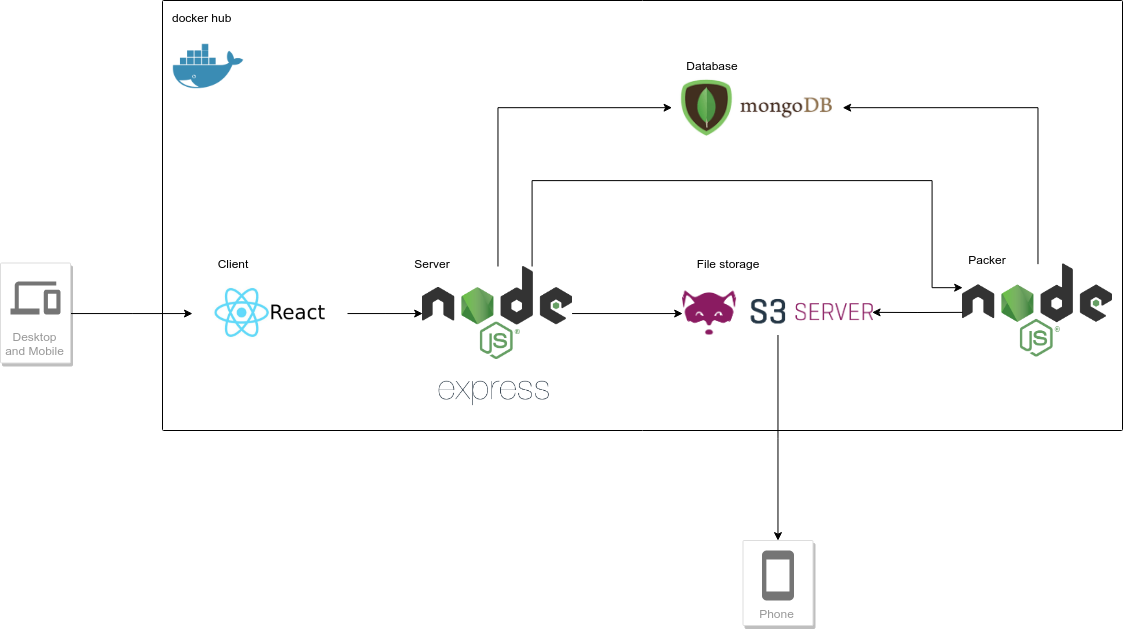
\includegraphics[width=1\textwidth]{img/3.png}
\captionsetup{justification=justified}
\caption{Результат проектирования. Архитектура разрабатываемого приложения и используемый стек технологий. }
\label{architecture_stack}
\end{figure}

\chapter{Разработка}

В этой главе описаны основные зависимости компонентов и принцип их действия. Приведены фрагменты кода и объяснено их действие. Описан процесс и резульаты тестирования для серверной части. Дано описание среды разработки.

\section{Среда разработки}

Используемая операционная система система и прикладные программы:
 
\begin{itemize}
	\item OS: Ubuntu 18.04 bionic
	\item Kernel: x86-64 Linux 4.15.0-50-generic
	\item IDE: Visual Studio Code
	\item Browser: Chromium v74.0.3729.108 (Official Build) snap (64-bit) and Firefox Quantum 66.0.5 (64-bit)
	\item Node.js v10.15.3
	\item npm v6.4.1
	\item Docker version 18.06.1-ce
	\item docker-compose version 1.22.0
\end{itemize}

\section{Серверная часть}

Для создания серверной части использовались платформа Node.js и фреймворк Express. Сервер обеспечивает взаимодействие клиента с базой данных, файловым хранилищем и упаковщиком.

Первоначальная структура проекта создавалось с помощью утилиты “express-generator”. Ключевой файл серверной части веб-приложение - это app.js. В его задачи входит установка соединений с базой данных, подключение cookie-сессий, и обработка запросов на различные url-адреса. Также в его задачу входит обработка ошибок. Поддерживается обработка ошибки с кодом 404 - “Не найдено” и ошибки с кодом 500 - “Ошибка сервера”.

При получении запроса сервер, в зависимости от того, на какой url запрос отправлен, задает файл обработчик. Например, в случае, когда запрос отправлен на корень сервера, его обработка в app.js будет выглядеть так:

\begin{lstlisting}[
    language=JavaScript,
    caption={Пример перенаправления обработки запроса на корень сервера для файла app.js}
]

const index = require("./routes/index");
       ...
app.use("/", index);

\end{lstlisting}

Обработка запроса перенаправляется в файл, index.js, который располагается в папке routes. Код расположенный в файле index.js:

\begin{lstlisting}[
    language=JavaScript,
    caption={Пример обработки запроса на корень сервера для файла index.js}
]

const express = require("express"),
      router = express.Router(),
      models = require("../models");

router.get("/", async (req, res) => {
  try {
    const id = req.session.userId;
    const login = req.session.userLogin;

    const courses = await models.Course.find({ published: true }).sort({
      createdAt: -1
    });

    res.json({
      courses,
      user: {
        id,
        login
      }
    });
  } catch (error) {
    throw new Error("Server Error");
  }
});

module.exports = router;

\end{lstlisting}


Сначала объявляются зависимости, используемые в файле. Далее задается обработчик GET-запроса, при url равному “/index”. Блок try-catch используется для корректной обработки исключений. Далее из запроса извлекаются id и login пользователя, а из базы данных все курсы, с поднятым флагом published, и сортировкой по убыванию для поля даты создания. Собранные данные отправляются клиенту, в JSON формате. Конструкция module.exports, позволяет экспортировать обработчик, чтобы его можно было подключить в файле app.js.

Полный список зависимостей серверной части представлен в файле package.json, но некоторые из них, которые являются ключевыми, описаны ниже:

\begin{itemize}
	\item aws-sdk - модуль, обеспечивающий доступ к файловому хранилищу, реализующему интерфейс AWS
	\item mongoose - ODM для MongoDB
	\item bindings и node-gyp - два модуля, позволяющие вызывать из JavaScript код на C++
	\item dotenv - модуль, позволяющий задавать параметры сервера, через переменные среды
	\item bcrypt-nodejs - библиотека позволяющая шифровать пароли
	\item cookie-session - позволяет использовать cookie для хранения пользовательских сессий
	\item multer - модуль, использующийся для обработки загрузки файлов
\end{itemize}

Также у серверной части приложения есть зависимости, которые необходимы лишь в процессе разработки:

\begin{itemize}
	\item mocha - фреймворк, позволяющий в асинхронном режиме запускать тесты
	\item chai и chai-http - BDD / TDD библиотека с функциями для проверки внутреннего состояния программы, а также модуль к этой библиотеке, который позволяет в удобной форме отправлять http-запросы
	\item nodemon - утилита, контролирующая изменения в коде и автоматически перезагружающая приложение
	\item eslint - инструмент для статического анализа кода
\end{itemize}

Используемые версии всех подключаемых модулей зафиксированы в файле package-lock.json.

\section{База данных}

В качестве СУБД используется MongoDB. Основная задача базы данных - это хранения информации о курсах и пользователях. Для информации хранения в базе данных используется 5 схем:

\begin{itemize}
	\item курсы
	\item уроки
	\item задачи
	\item пользователи
	\item опубликованные курсы.
\end{itemize}

Курсы, уроки и задачи хранят данные характеризующие контент создаваемый для мобильной среды. Схема с пользователями используется для хранения пароля в зашифрованном виде и логина. Схема опубликованные курсы, хранит краткое описание курсов, ссылки, по которым можно скачать архив курса и дату публикации. Схемами курсы, уроки, задачи и пользователи пользуется для чтения и редактирования серверная часть. Упаковщик пользуется курсами, уроками, задачами для чтения, а опубликованными курсами для чтения и записи.

\section{Клиентская часть}

Для создания клиентской части использовался язык JavaScript и фреймворк React. Компонент, получающий данные в JSON виде с серверной части, обеспечивающий формирование пользовательского интерфейса и отображение его в браузере пользователя. Приложение запускается на отдельном сервере, который проксирует запросы на файловое хранилище и основной сервер. Клиентская часть создана на одностраничной архитектуре. 

Для того, чтобы обеспечить обновление контента без перезагрузки страницы используется React компонент BrowserRouter. Он позволяет посылать различные url запросы, не перезагружая страницу. Ниже представлен код, позволяющие в зависимости от url запроса демонстрировать либо страницу для отображения курса, либо страницу для его редактирования.


\begin{lstlisting}[
    language=JavaScript,
    caption={Пример кода компонента Клиент, демонстрирующий механизм роутинга}
]

<Switch>
  <Route exact path="/content/course/:courseId" render={(props) => (
    <Paper className={classes.paper}>
      <ContentCourse {...props} accId={this.props.accId} />
    </Paper>
  )} />
	
  <Route exact path="/content/edit/course/:courseId" render={(props) => (
    <Paper className={classes.paper}>
      <EditCourse {...props} accId={this.props.accId} />
    </Paper>
  )} />
      ...
</Switch>

\end{lstlisting}



Для создания графического интерфейса, помимо основополагающего фреймворка React, используется React-библиотека Material-UI\footnote{https://material-ui.com/}, которая предоставляет набор визуальных решений, соответствующих принципам Material Design. Для визуализации аудиофайла использовалась библиотека wavesurfer.js\footnote{https://wavesurfer-js.org/}, а для визуализации файла с питчом библиотека dygraphs\footnote{http://dygraphs.com/}.

На рисунках \ref{gui_1}, \ref{gui_2}, \ref{gui_3}, \ref{gui_4} представлен разработанный графический интерфейс приложения.

\newpage

\begin{figure}[H]
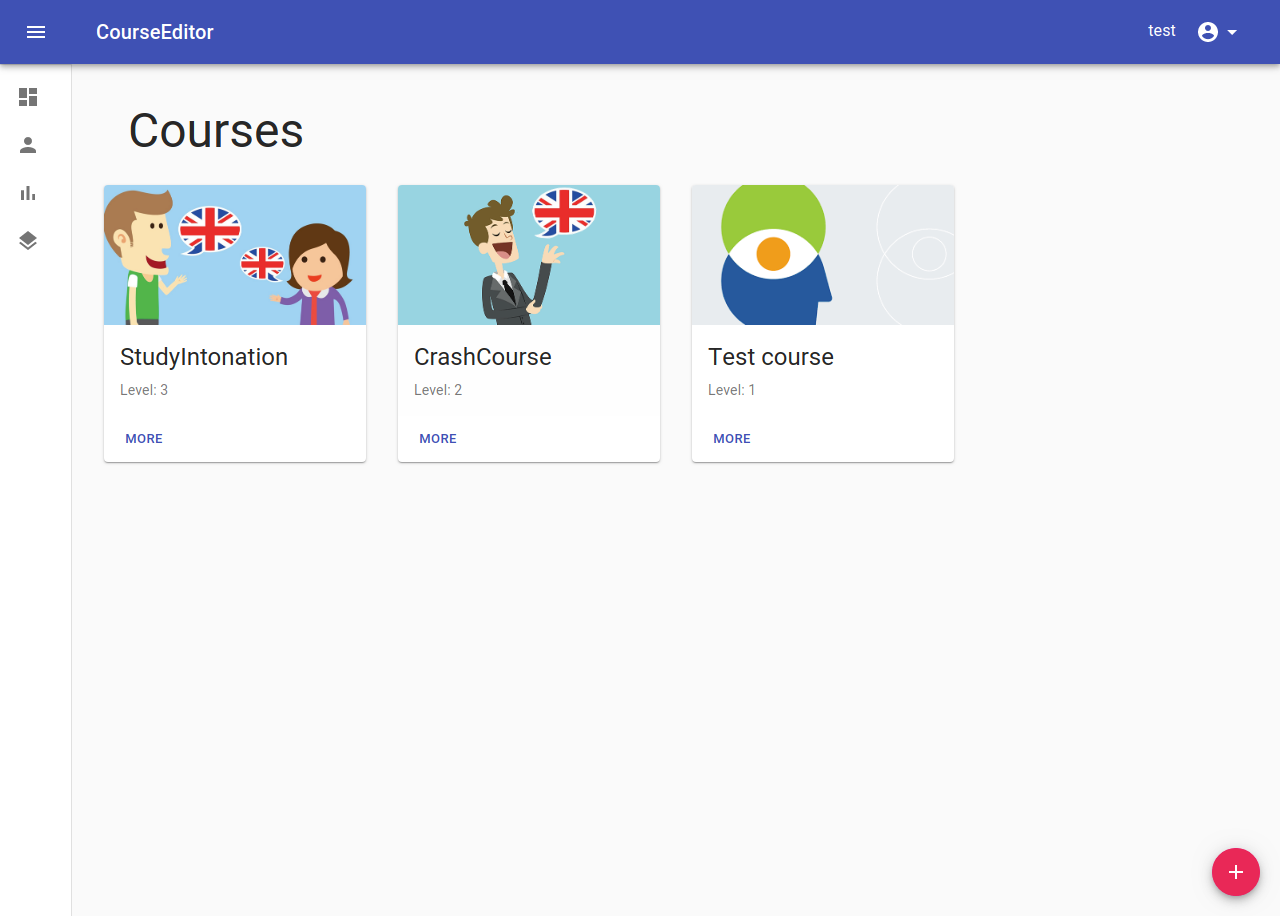
\includegraphics[width=0.8\textwidth]{img/5.png}
\captionsetup{justification=justified}
\caption{Графический интерфейс приложения. Desktop версия. Экран с курсами.}
\label{gui_1}
\end{figure}

\begin{figure}[H]
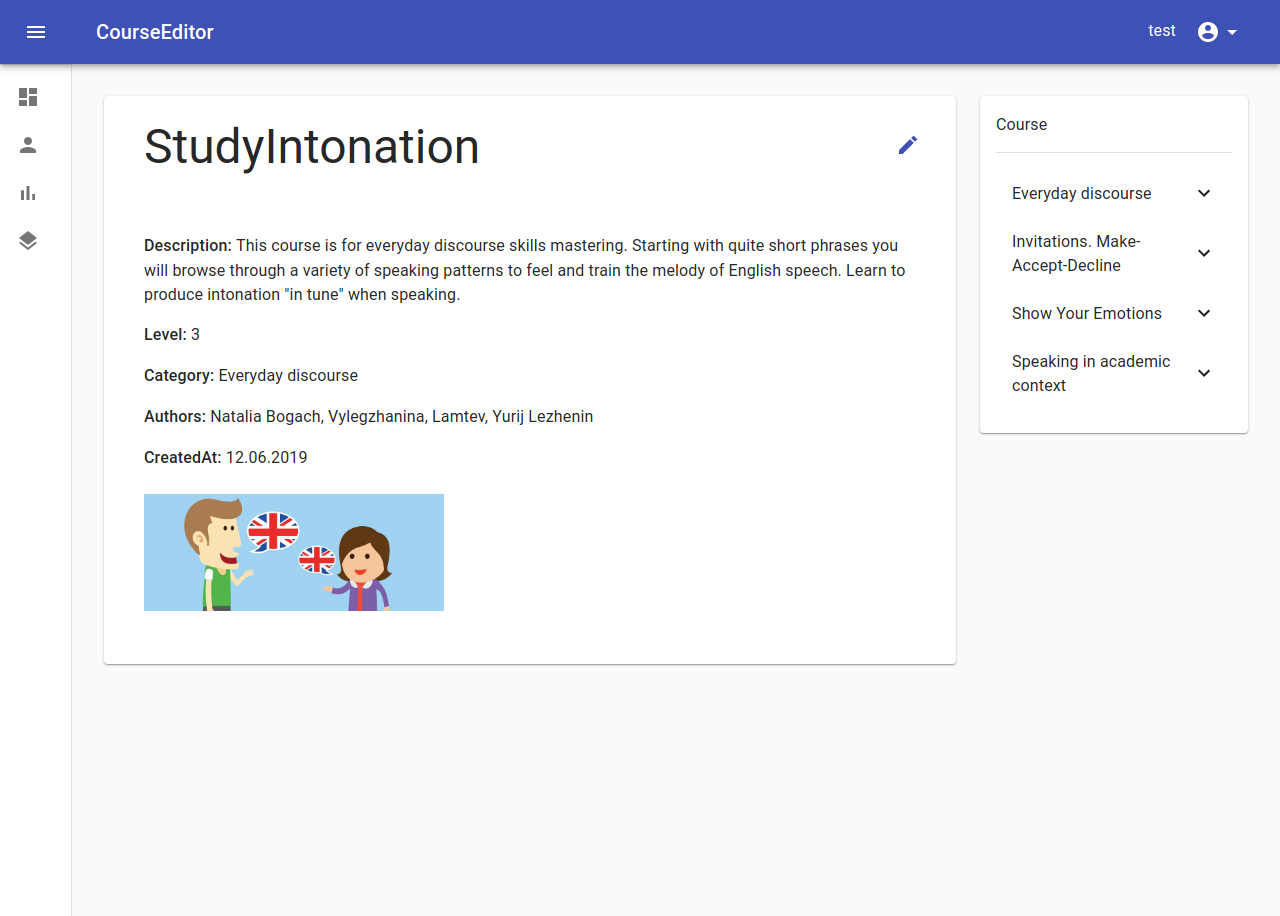
\includegraphics[width=0.8\textwidth]{img/6.png}
\captionsetup{justification=justified}
\caption{Графический интерфейс приложения. Desktop версия. Экран с курсом.}
\label{gui_2}
\end{figure}
 
\begin{figure}[H]
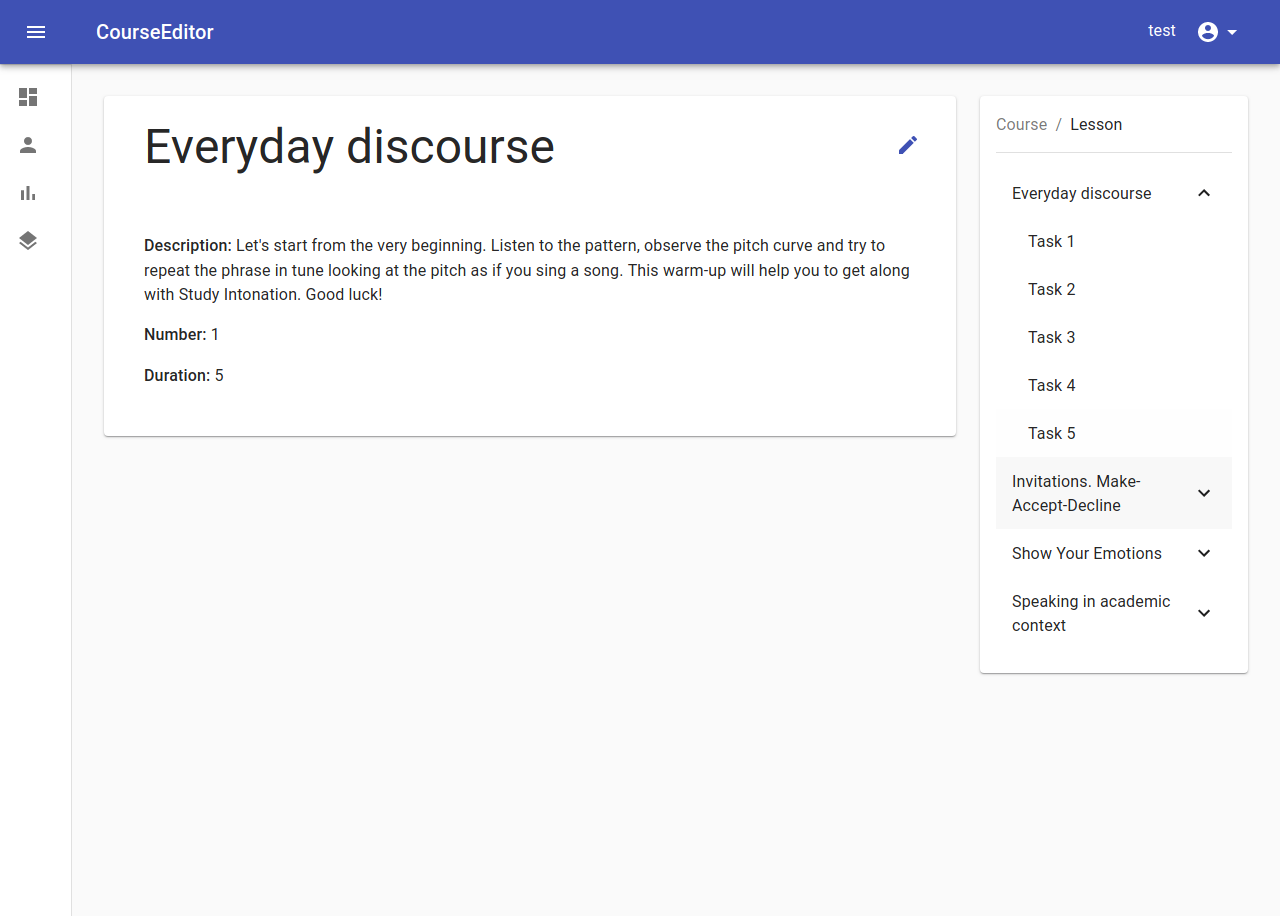
\includegraphics[width=0.8\textwidth]{img/7.png}
\captionsetup{justification=justified}
\caption{Графический интерфейс приложения. Desktop версия. Экран с уроком.}
\label{gui_3}
\end{figure}

\begin{figure}[H]
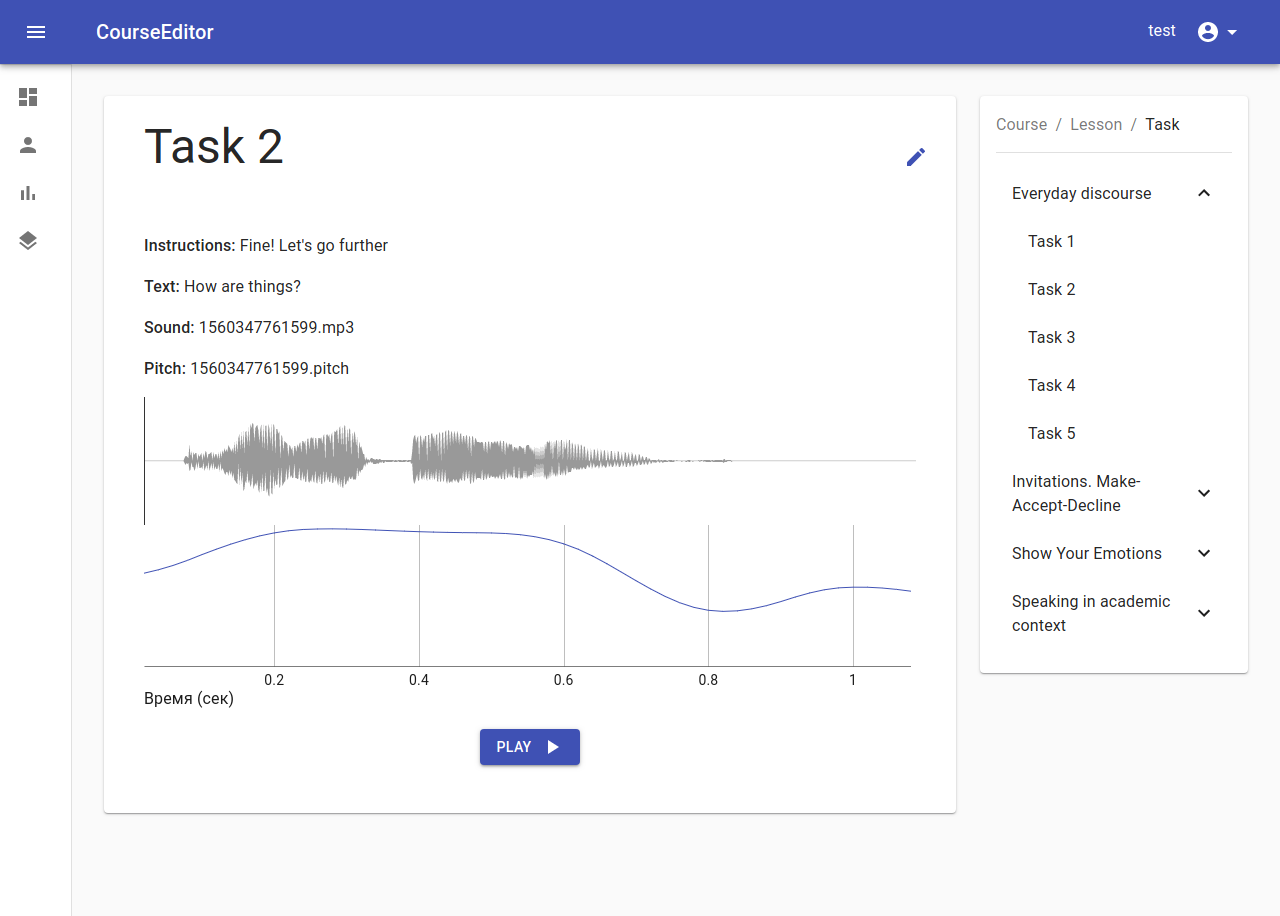
\includegraphics[width=0.8\textwidth]{img/8.png}
\captionsetup{justification=justified}
\caption{Графический интерфейс приложения. Desktop версия. Экран с задачей.}
\label{gui_4}
\end{figure}

Предусмотрена валидация полей при редактировании и создании контента.
Для информирования пользователей о некорректном вводе используются всплывающие уведомления и подсветка форм, в которых допущена ошибка.
На рисунке \ref{gui_5} продемонстрирована ошибка - незаполненное поле.

\begin{figure}[H]
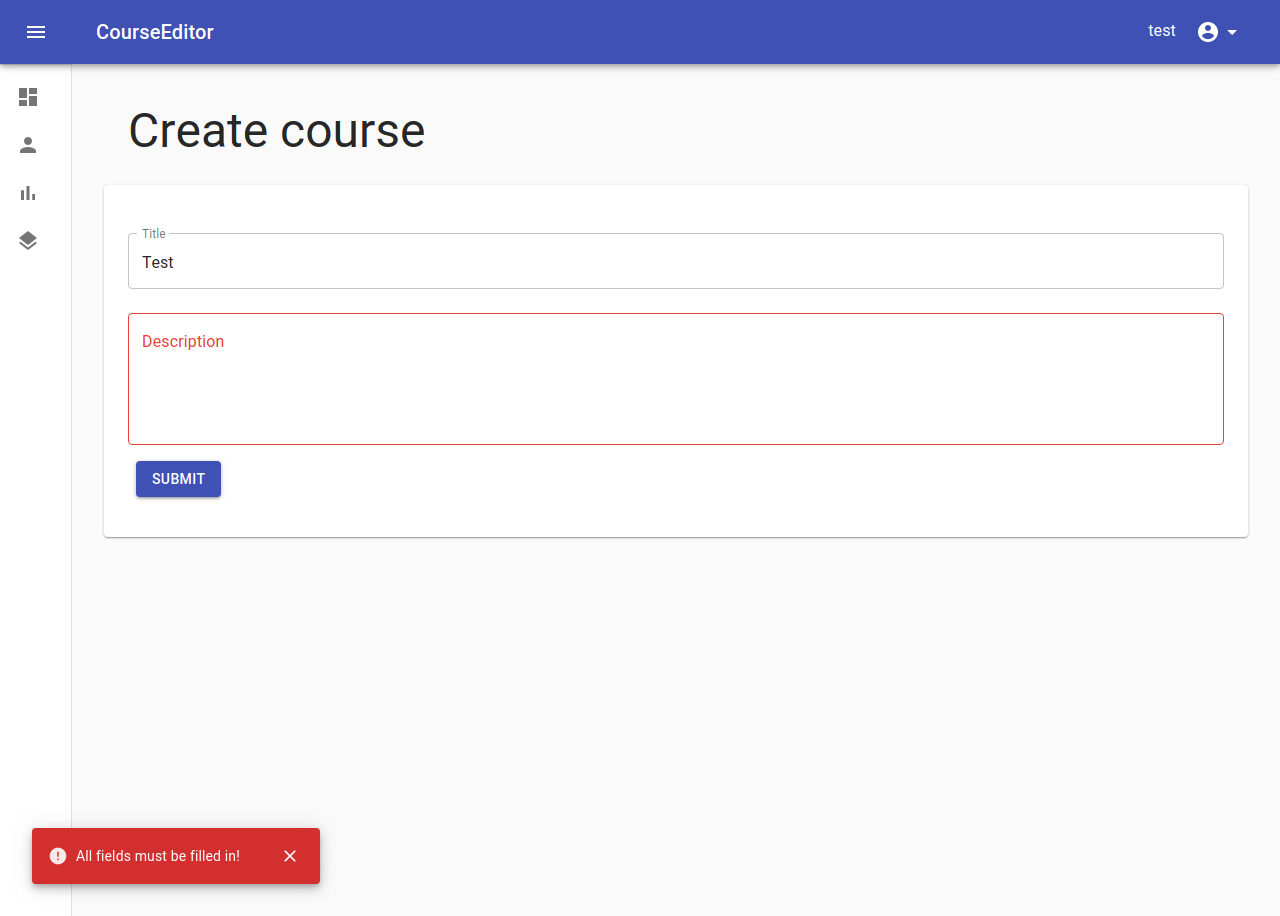
\includegraphics[width=0.8\textwidth]{img/9.png}
\captionsetup{justification=justified}
\caption{Графический интерфейс приложения. Desktop версия. Экран с уведомлением о некорректном заполнении формы.}
\label{gui_5}
\end{figure}

\newpage

Разработанное веб-приложение является адаптивным и правильно отображается на устройствах, с разными размерами экрана. На рисунке \ref{gui_6} продемонстрировано отображение мобильной версии веб-приложения.

\begin{figure}[H]
\begin{minipage}[H]{0.49\linewidth}
\center{
\includegraphics[width=1\linewidth]{img/10.png} \\ а) Экран с курсами}
\end{minipage}
\hfill
\begin{minipage}[H]{0.49\linewidth}
\center{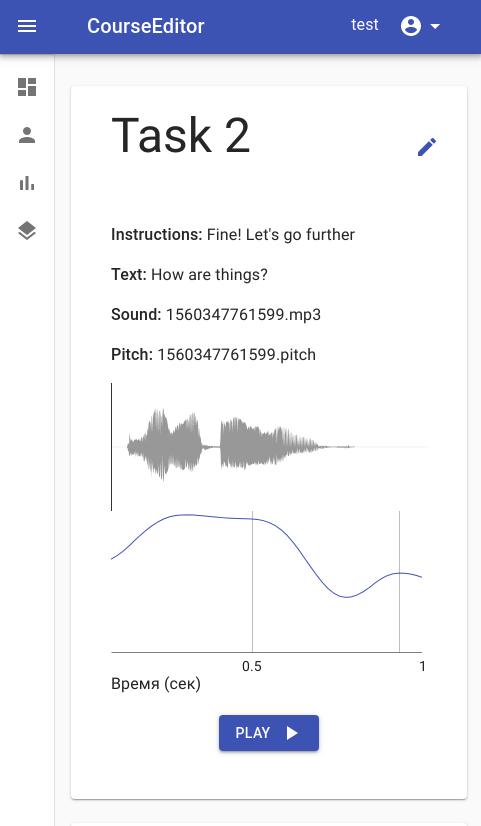
\includegraphics[width=1\linewidth]{img/11.png} \\ б) Экран с задачей}
\end{minipage}
\caption{Графический интерфейс приложения. Мобильная версия.}
\label{gui_6}
\captionsetup{justification=justified}
\end{figure}
 
На стороне клиента организована аутентификация и авторизация. Приложение не допускает пользователя до экрана создания или редактирования курса, пока он пройдет не аутентификацию.

\section{Упаковщик}

Для реализации этого компонента используется Node.js. Эта часть приложения, отвечающая за сбор данных по выбранному курсу и формированию архива из них, а также формирования файла с информацией о всех доступных для скачивания курсов, который носит название info.json.
Ключевыми зависимостями этого компонента, являются:

\begin{itemize}
	\item archiver - библиотека, для архивирования, в данном случае используются zip-архивы
	\item sha256 - библиотека для вычисления hash-кода для архива, результат вычисления размещается в поле описания курса в файле info.json и необходим для корректного скачивания курса
\end{itemize}

Остальные зависимости приведены в файле package.json для этого компонента.

\section{Файловое хранилище}

В качестве реализации файлового хранилища используется Scality S3 Server.
Ниже приведен фрагмент кода файла docker-compose.yml для файлового хранилища:


\begin{lstlisting}[
    language=JavaScript,
    caption={Фрагмент файла docker-compose.yml для компонента Файловое хранилище}
]

  scality:
    image: scality/s3server
    ports:
      - 8080:8000
    volumes:
      - ./scality/config.json:/usr/src/app/config.json
    environment:
      SCALITY_ACCESS_KEY_ID: '12340'
      SCALITY_SECRET_ACCESS_KEY: '01234560'
      SSL: 'FALSE'

\end{lstlisting}

Через среду окружения задаются два ключа доступа. Для компонентов, которые взаимодействуют с файловым хранилищем указываются такие же ключи, после этого для них разрешаются операции на запись.

\section{Докеризация}

При проектировании было выделено 5 докеров под клиентскую часть, серверную, упаковывающее приложение, базу данных и файловое хранилище.
Пример docker-файла для упаковщика:


\begin{lstlisting}[
    language=JavaScript,
    caption={Содержимое Docker-файла для компонента Упаковщик}
]

FROM node:8

ENV NODE_ENV development
ENV PORT 8080
ENV MONGO_URL mongodb://localhost:27017/course-editor

WORKDIR /course-packer
ADD . .

RUN npm install

ENTRYPOINT npm start

\end{lstlisting}

Для запуска контейнеров и организации связей между ними используется docker-compose. В docker-compose прописаны зависимости от двух сторонних docker-образ:

\begin{itemize}
	\item mongo - образ с базой данных MongoDB
	\item scality/s3server - образ с файловым хранилищем S3 server, реализующем AWS интерфейс 
\end{itemize}

Запуск приложения осуществляется с помощью команды docker-compose up. После этого скачиваются и устанавливаются все Docker-образы описанные в файле docker-compose.yml и происходит запуск веб-приложения. 

\section{Тестирование}

Для тестирования сервера использовались JavaScript-библиотеки Mocha\footnote{https://mochajs.org/} и Chai\footnote{https://www.chaijs.com/}. Mocha, как основной фреймворк для тестирования и Chai, как библиотека для формирования http-запросов и проверки их результатов. Для вычисления покрытия кода тестами использовалась библиотека nyc.

\begin{lstlisting}[
    language=JavaScript,
    caption={Пример теста, который проверяет корректность механизма валидации данных}
]

it('POST /auth/registration (error: "All fields must be filled in!" for 2 fields)', done => {
     chai
     .request(server)
     .post("/auth/registration")
     .type('form')
     .send({
       'login': 'name'
     })
     .end((err, res) => {
       res.should.have.status(200);
       res.should.be.json;
       res.body.ok.should.be.false;
       res.body.error.should.be.equal("All fields must be filled in!");
       res.body.fields.should.have.members(['password', 'passwordConfirm']);
       done();
     });
});
\end{lstlisting}

На сервер отправляется POST запрос по url “/auth/registration”. Запрос содержит форму, форма одно поле. Ожидается, что сервер вернёт 200 код, что будет свидетельствовать об успешной обработке запроса. Тело ответа должно быть в формате JSON и должно содержать сообщение об ошибке, что какое-то поле не заполнно. Также ожидается, что в ответе содержатся идентификаторы полей, которые не устроили сервер.

Выделено 104 теста, каждый из которых отвечает за покрытие отведенной функциональности сервера. Тесты объединены в 5 групп: 

\begin{itemize}
	\item Создание пользователя и его аутентификация
	\item Создание и проверка на доступность для курсов, уроков и задач
	\item Редактирование и удаление курсов, уроков, задач
	\item Загрузка медиафайлов(изображений и звуковых файлов)
	\item Обработка некорректных запросов к серверу
\end{itemize}

Библиотека для вычисления покрытия кода тестами nyc, позволяет считать покрытие по 4-м метрикам. В качестве результирующего значение берётся средние из посчитаных величин.

В итоге тестирования был получен следующий результат:

Файлы, где покрытие по некоторым метрикам опускается ниже 80\%, можно объяснить невозможностью достичь определенных участков кода в связи с тем, что в них используется переключение между тестовым и реальным режимами.

\begin{figure}[H]
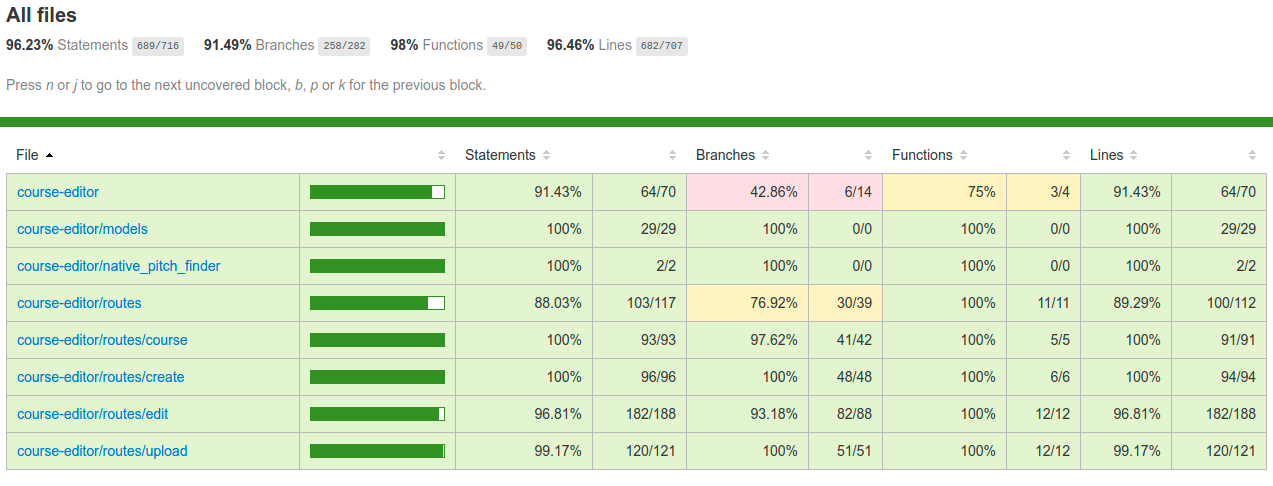
\includegraphics[width=1\textwidth]{img/4.png}
\captionsetup{justification=justified}
\caption{Результаты тестирования.}
\label{test_reslut}
\end{figure}

В процессе тестирования были выявлены ошибки связанные с некорректной обработкой запросов. На сервер отправлялись запросы с несуществующим идентификатором курса, из-за неправильной последовательности разбора случался сбой.

Код размещается в gitlab репозитории. После каждого обновления кода в репозитории происходит запуск тестов и вычисляется покрытие кода. Для реализации непрерывной интеграции используется Gitlab CI. 

\section{Результаты}

В результате разработки было получено веб-приложение состоящее из 5 докеров (клиент, сервер, база данных, упаковщик, файловое хранилище) и сформирован docker-compose файл, позволяющий разворачивать приложение.

Разработан набор тестов обеспечивающий покрытие кода серверной части свыше 90\%. Docker контейнеры и сервис Gitlab CI позволяют запускать тесты и вычислять покрытие, после каждого обновления кода в репозитории.

Проект состоит из 5 компонентов. Серверная часть состоит из 49 файлов, а клиентская из 31 файла. Упаковщик состоит из 13 файлов.

\conclusion

Работа разделена на 3 главы, отражающие жизненный цикл разработки программного обеспечения: анализ предметной области, заключающийся в обзоре существующих решений, и разработка необходимых требований, предъявляемых к продукту; проектирование архитектуры, включающее в себя выбор технологического стека; реализация конечного продукта с дальнейшим тестированием.

В ходе работы определено место продукта в предметной области. Сформулирована мотивация разработки собственного решения. 
Цель работы достигнута. Веб-приложение, позволяющее создавать, редактировать и распространять курсы по изучению интонации для пользователей проекта “Study Intonation” разработано успешно. Функциональные и нефункциональные требования, предъявляемые к продукту, выполнены. Освоен процесс разработки одностраничного веб-приложения, получен опыт реализации приложений на технологическом стеке MERN + AWS S3, а также опыт работы с Docker-контейнерами.


\bibliography{thesis} 
\bibliographystyle{ugost2008s}

\appendix
\nchapter{ПРИЛОЖЕНИЕ 1. ЛИСТИНГИ}

\begin{lstlisting}[
    language=JavaScript,
    caption={Компонент - Сервер, файл course/course.js, содержащий обработку 2 запросов}
]

const express = require("express"),
      router = express.Router(),
      request = require('request'),
      models = require("../../models");

router.get("/:courseId", async (req, res, next) => {
  const userLogin = req.session.userLogin;
  const userId = req.session.userId;

  const courseId = req.params.courseId;

  if (!courseId.match(/^[0-9a-fA-F]{24}$/)) {
    const err = new Error("Not Found");
    err.status = 404;
    next(err);
  } else {
    const course = await models.Course.findById(courseId);
    if (!course) {
      const error = new Error("Not Found");
      error.status = 404;
      next(error);
    } else if (
      !course.published &&
      (!userLogin || !userId || userId != course.owner)
    ) {
      res.json({
        ok: false,
        error: 'Forbidden',
      });
    } else {
      res.json({
        ok: true,
        course,
      });
    }
  }
});

router.get("/publish/:courseId", async (req, res, next) => {
  const userLogin = req.session.userLogin;
  const userId = req.session.userId;

  const courseId = req.params.courseId;

  if (!courseId.match(/^[0-9a-fA-F]{24}$/)) {
    const err = new Error('Not Found');
    err.status = 404;
    next(err);
  } else {
    const course = await models.Course.findById(courseId);

    if (!course) {
      const error = new Error('Not Found');
      error.status = 404;
      next(error);
    } else if (
      !course.published &&
      (!userLogin || !userId || userId != course.owner)
    ) {
      res.json({
        ok: false,
        error: 'Forbidden',
      });
    } else {
      request.post('http://course-packer:8000/course').form({id:courseId});
      res.json({
        ok: true,
        url: `/uploads/${courseId}.zip`,
      })
    }
  }
});

module.exports = router;

\end{lstlisting}



\begin{lstlisting}[
    language=JavaScript,
    caption={Компонент - Сервер, файл edit/course.js, содержащий обработку 2 запросов}
]

const express = require("express"),
      router = express.Router(),
      models = require("../../models"),
      util = require("../utils");

router.post('/', async (req, res, next) => {
  const userLogin = req.session.userLogin;
  const userId = req.session.userId;

  const courseId = req.body.id;
  const course = await models.Course.findById(courseId);
  if (!course) {
    var err = new Error('Not Found');
    err.status = 404;
    next(err);
  } else if (!userLogin || !userId || userId != course.owner) {
    res.json({
      ok: false,
      error: 'Forbidden',
    });
  } else {
    let {
      title,
      description,
      complexity,
      category,
      authors,
      published
    } = req.body;

    if (!title) {
      title = course.title;
    }
    if (!description) {
      description = course.description;
    }
    if (!complexity) {
      complexity = course.complexity;
    }
    if (!category) {
      category = course.category;
    }
    if (!authors) {
      authors = course.authors;
    }
    if (!published) {
      published = course.published;
    }

    const newCourse = await models.Course.findOneAndUpdate(
      {
        _id: course.id,
        owner: userId
      },
      {
        title,
        description,
        complexity,
        category,
        authors,
        owner: userId,
        published
      },
      { new: true }
    );

    if (!newCourse) {
      res.json({
        ok: false,
        error: 'Something went wrong'
      });
    } else {
      res.json({
        ok: true
      });
    }
  }
});

router.delete('/', async (req, res, next) => {
  const userLogin = req.session.userLogin;
  const userId = req.session.userId;

  const courseId = req.body.id;
  const course = await models.Course.findById(courseId);
  if (!course) {
    var err = new Error('Not Found');
    err.status = 404;
    next(err);
  } else if (!userLogin || !userId || userId != course.owner) {
    res.redirect("/");
  } else {
    var removedTasksOK = true;
    const lessons = await models.Lesson.find({ course: courseId });
    lessons.forEach(async lesson => {
      const tasks = await models.Task.find({ lesson: lesson.id });
      tasks.forEach( task => {
        util.removeUploadsFromS3(task.sound);
        util.removeUploadsFromS3(task.pitch);
      });
      const removedTasks = await models.Task.deleteMany({ lesson: lesson.id });
      removedTasksOK = removedTasksOK && removedTasks.ok;
    });
    const removedLessons = await models.Lesson.deleteMany({ course: course.id });
    util.removeUploadsFromS3(course.logo);
    const removedCourse = await models.Course.findByIdAndRemove(course.id);

    if (!removedCourse || !removedLessons.ok || !removedTasksOK) {
      res.json({
        ok: false,
        error: 'Something went wrong'
      });
    } else {
      res.json({
        ok: true
      });
    }
  }
});

module.exports = router;


\end{lstlisting}




\begin{lstlisting}[
    language=JavaScript,
    caption={Компонент - Сервер, файл image.js содержащий обработку загрузки изображений}
]

const express = require("express"),
      router = express.Router(),
      path = require("path"),
      multer = require("multer"),
      multerS3 = require('multer-s3'),
      AWS = require("aws-sdk"),
      config = require("../../config"),
      models = require("../../models"),
      util = require("../utils");

const s3 = new AWS.S3(config.AWS_PARAM);
const storage = multerS3({
  s3: s3,
  bucket: config.DESTINATION,
  acl: 'public-read',
  contentType: multerS3.AUTO_CONTENT_TYPE,
  key: async (req, file, cb) => {
    const userLogin = req.session.userLogin;
    const userId = req.session.userId;

    const courseId = req.body.courseId;
    const course = await models.Course.findById(courseId);

    if (!course) {
      let err = new Error('Not Found');
      err.code = 'NOCOURSE';
      cb(err);
    } else if (!userLogin || !userId || userId !=
      course.owner) {
      let err = new Error('Is not allowed');
      err.code = 'NOTALLOWED';
      cb(err);
    } else {
      if (course.logo !== 'none') {
        util.removeUploadsFromS3(course.logo);
      }
      const filePath = Date.now() + path.extname(file.originalname);
      await models.Course.findOneAndUpdate(
        {
          _id: course.id,
          owner: userId
        },
        {
          logo: filePath
        },
        { new: true }
      );      
      cb(null, filePath);
    }
  }
});

const upload = multer({
  storage,
  fileFilter: (req, file, cd) => {
    const ext = path.extname(file.originalname);
    if (ext !== '.jpg' && ext !== '.jpeg' && ext !== '.png') {
      const err = new Error('Extention');
      err.code = 'EXTENTION';
      return cd(err);
    }
    cd(null, true);
  },
  limits: {
    fileSize: 3 * 1024 * 1024,
  },
}).single('file');

router.post('/', (req, res) => {
  upload(req, res, err => {    
    let error = '';
    if (err) {
      console.log(err);      
      if (err.code === 'EXTENTION') {
        error = 'Only jpeg and png!';
      }
      if (err.code === 'NOCOURSE') {
        error = 'Nothing found!';
      }
      if (err.code === 'NOTALLOWED') {
        error = 'Invalid auth!';
      }
      if (err.code === 'LIMIT_FILE_SIZE') {
        error = 'Limit file size!';
      }
      if (err.code === 'NoSuchBucket') {
        util.createBucketS3(config.DESTINATION);
        error = 'No such Bucket, pls, try again.';
      }
    }
    res.json({
      ok: !err,
      error
    });
  });
});

module.exports = router;


\end{lstlisting}

\begin{lstlisting}[
    language=JavaScript,
    caption={Компонент - Сервер, файл image.js содержащий обработку загрузки изображений}
]

FROM node:8

ENV NODE_ENV development
ENV PORT 8080
ENV MONGO_URL mongodb://localhost:27017/course-editor

WORKDIR /course-packer
ADD . .

RUN npm install

ENTRYPOINT npm start

\end{lstlisting}

\begin{lstlisting}[
    language=JavaScript,
    caption={Компонент - Сервер, файл my.js содержащий обработку запроса на курсы, принадлежащие пользователю}
]

const express = require("express"),
      router = express.Router(),
      models = require("../models");

router.get("/", async (req, res) => {
  try {
    const userId = req.session.userId;
    const userLogin = req.session.userLogin;

    const courses = await models.Course.find({ owner: userId }).sort({
      createdAt: -1
    });

    if (!userLogin || !userId) {
      res.json({
        ok: false,
        error: 'Forbidden',
      })
    } else {
      res.json({
        ok: true,
        courses,
      });
    }
  } catch (error) {
    throw new Error("Server Error");
  }
});

module.exports = router;

\end{lstlisting}

\begin{lstlisting}[
    language=JavaScript,
    caption={Компонент - Сервер, файл config.js содержащий конфигурационные параметры для серверной части}
]
const dotenv = require("dotenv");
const path = require("path");

const root = path.join.bind(this, __dirname);
dotenv.config({ path: root(".env") });

let mongoURL = "";
if (process.env.NODE_ENV == "test") {
  mongoURL = process.env.TEST_MONGO_URL;
} else {
  mongoURL = process.env.MONGO_URL;
}

const AWS_PARAM = {
  accessKeyId: process.env.ACCESS_KEY_ID,
  secretAccessKey: process.env.SECRET_ACCESS_KEY,
  endpoint: 'scality:8000',
  sslEnabled: false,
  s3ForcePathStyle: true
};

module.exports = {
  MONGO_URL: mongoURL,
  SESSION_SECRET: process.env.SESSION_SECRET,
  DEBUG: process.env.NODE_ENV === "development",
  PORT: process.env.PORT || 3000,
  DESTINATION: "uploads",
  AWS_PARAM
};

\end{lstlisting}

\begin{lstlisting}[
    language=JavaScript,
    caption={Компонент - Сервер, ключевой файл app.js, обеспевивающий подключение основных модулей и перенаправляющий обработку запросов}
]

const express = require("express"),
      path = require("path"),
      favicon = require("static-favicon"),
      logger = require("morgan"),
      cookieParser = require("cookie-parser"),
      bodyParser = require("body-parser"),
      proxy = require("express-http-proxy");

const index = require("./routes/index"),
      create = require("./routes/create"),
      edit = require("./routes/edit"),
      auth = require("./routes/auth"),
      course = require("./routes/course/course"),
      lesson = require("./routes/course/lesson"),
      task = require("./routes/course/task"),
      upload = require("./routes/upload"),
      myCourses = require("./routes/my"),
      info = require("./routes/info");

const staticAsset = require("static-asset");

const config = require("./config");

const cookieSession = require('cookie-session');

// database
const mongoose = require("mongoose");
mongoose.set("debug", config.DEBUG);
mongoose.connect(
  config.MONGO_URL,
  { useNewUrlParser: true }
);

const db = mongoose.connection;
db.on("error", console.error.bind(console, "Connection error:"));
db.once("open", function() {
  if (config.DEBUG) {
    console.log("Connection to database open.");
  }
});

// express
const app = express();

app.use(cookieSession({
  name: 'session',
  keys: [config.SESSION_SECRET]
}));

// view engine setup
app.set("views", path.join(__dirname, "views"));
app.set("view engine", "ejs");

if (process.env.NODE_ENV !== 'test') {
  app.use(logger("dev"));
}

app.use(favicon());
app.use(bodyParser.json());
app.use(bodyParser.urlencoded({ extended: true }))
app.use(cookieParser());
app.use(staticAsset(path.join(__dirname, "public")));
app.use(express.static(path.join(__dirname, "public")));

app.use('/uploads', proxy('scality:8000', {
  proxyReqPathResolver: (req) => {
    return '/uploads' + req.url;
  }
}));

app.use("/", index);
app.use("/create", create);
app.use("/edit", edit);
app.use("/auth", auth);
app.use("/course", course);
app.use("/lesson", lesson);
app.use("/task", task);
app.use("/upload", upload);
app.use("/my", myCourses);
app.use("/info", info);

/// catch 404 and forwarding to error handler
app.use(function(req, res, next) {
  var err = new Error('Not Found');
  err.status = 404;
  next(err);
});

/// error handlers

// development error handleenvr
// will print stacktrace
if (app.get('env') === 'development') {
  app.use(function(err, req, res, next) {
    res.status(err.status || 500);
    res.json({
      message: err.message,
      error: err
    });
  });
}

// production error handler
// no stacktraces leaked to user
app.use(function(err, req, res, next) {
  res.status(err.status || 500);
  res.json({ 
    message: err.message,
    error: {}
  });
});

module.exports = app;

\end{lstlisting}

\begin{lstlisting}[
    language=JavaScript,
    caption={Компонент - Клиент, файл App.js}
]

import React, {Component} from 'react';
import CourseEditor from './components/CourseEditor';
import { BrowserRouter } from 'react-router-dom';

class App extends Component {

  render() {
    return (
      <div className="App">

        <BrowserRouter>

          <CourseEditor />
          
        </BrowserRouter>
        
      </div>
    );
  }
}

export default App;


\end{lstlisting}

\begin{lstlisting}[
    language=JavaScript,
    caption={Компонент - Клиент, файл Courses.js}
]

import React, {Component} from 'react';
import Grid from '@material-ui/core/Grid';
import Typography from '@material-ui/core/Typography';
import { withStyles } from '@material-ui/core/styles';
import Fab from '@material-ui/core/Fab';
import AddIcon from '@material-ui/icons/Add';
import { Link } from 'react-router-dom';
import Card from './MediaCard';
import utils from '../utils';

const styles = theme => ({
  title: {
    marginTop: theme.spacing(1),
    marginBottom: theme.spacing(4),
    marginLeft: theme.spacing(3),
  },
  fab: {
    margin: 0,
    top: 'auto',
    right: 20,
    bottom: 20,
    left: 'auto',
    position: 'fixed',
    'z-index': 999, 
  },
});

class Courses extends Component {
  state = {courses: []};

  componentDidMount() {
    utils.callApi('/index')
      .then(res => this.setState({courses: res.courses}))
      .catch(err => console.log(err));
  }

  CoursesCards = () => {    
    if (this.state.courses.length === 0) {
      return (
        <div>
          <p>
            There are no courses, but you should rejoice!
          </p>
        </div>
      )
    } else {
      return (
        <Grid container spacing={4}>
          {this.state.courses.map( course =>
            <Card key={course.id} course={course}/>
          )}
        </Grid>
      )
    }
  }

  render() {
    return (
      <div className="container">
        <Typography component="h1" variant="h3" color="inherit" className={this.props.classes.title}>
          Courses
        </Typography>

        { 
          this.props.auth ?
            <Link
              to='/create/course'
              className={this.props.classes.fab}
            >
              <Fab
                size="medium"
                color="secondary"
                aria-label="Add" 
              >
                  <AddIcon />
              </Fab>
            </Link>
          :
            null
        }

        <this.CoursesCards className={this.props.classes.lol}/>
        
      </div>
    );
  }
}

export default withStyles(styles)(Courses);

\end{lstlisting}


\end{document}

%%%%%%%%%%%%%%%%%%%%%%%%%%%%%%%%%%%%%%%%%%%%%%%%%%%%%%%%%%%%%%%%%%%%%%%%%%%%%%%%
